\documentclass{beamer}
\usetheme{Frankfurt}
\usepackage{tikz}
\usepackage{minted}
\usefonttheme{professionalfonts}
\usecolortheme{sidebartab}
\usepackage{xcolor}
\usepackage{hyperref}

\usetikzlibrary{chains, shadows.blur, trees}
%Information to be included in the title page:
\title[\url{https://google.com}] %optional
{LLVM \& HPSSA}

\subtitle{Hot Path SSA Form in LLVM}

\author[VIP1 \& VIP2] % (optional, for multiple authors)
{Presented By Abhay\inst{1} \& Muzzammil\inst{1}}

\institute[IDK] % (optional)
{
	\inst{1}%
	IIT Kanpur\\
	PRAISE Group
}

\date[01/03/2022] % (optional)
{Dr. Subhajit Roy, Dr. Awanish Pandey, Mr. Sumit Lahiri}

\begin{document}
\frame{\titlepage}

\section{LLVM Modifications}

\begin{frame}
	\frametitle{What we modified in LLVM?}
	\begin{itemize}
		\item New \mintinline[]{css}{llvm::intrinsic} signature, \mintinline[]{css}{"llvm.tau"}.
		\item Modified \mintinline[]{css}{Verifier::verifyDominatesUse()} since we don't want our intrinsic to interfere with \mintinline[]{css}{dominators} computation.  
	\end{itemize}
\end{frame}

\begin{frame}
	\frametitle{What we modified in LLVM?}
	\begin{itemize}
		\item New \mintinline[]{css}{llvm::intrinsic} signature, \mintinline[]{css}{"llvm.tau"}.
		\item Modified \mintinline[]{css}{Verifier::verifyDominatesUse()} since we don't want our intrinsic to interfere with \mintinline[]{css}{dominators} computation.  
	\end{itemize}
\end{frame}


\section{LLVM : HPSSA Pass}

\begin{frame}
	\frametitle{\texttt{HPSSAPass} : Overview}
	\begin{itemize}
		\item New \mintinline[]{css}{llvm::HPSSAPass} pass using the new Pass Manager. 
		\item Pass runs over a \mintinline[]{css}{llvm::Function} and inserts \mintinline[]{css}{"llvm.tau"} intrinsic calls with speculative and safe arguments.
	\end{itemize}
	Key HPSSA Data Structures :  
	\begin{itemize}
		\item Hot Path Set using \mintinline[]{css}{llvm::BitVector}.
		\item Definition Accumalator, \texttt{defAccumalate} as a map  \mintinline[]{python}{std::map<{PHINode*,BasicBlock*}, {Value*,BitVector}>}.
		\item Variable Renaming Stack as a map, \mintinline[]{python}{std::map<Value*,Value*>}
	\end{itemize}
\end{frame}

\begin{frame}{HPSSA Transformation}
	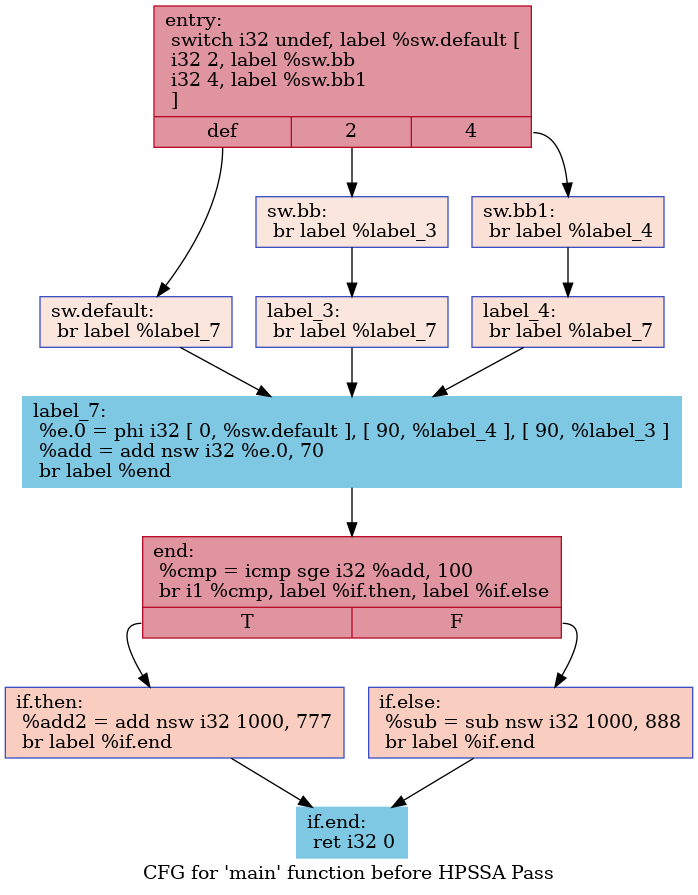
\includegraphics[width=4.8cm,height=7.5cm]{baseline.dot.png}
	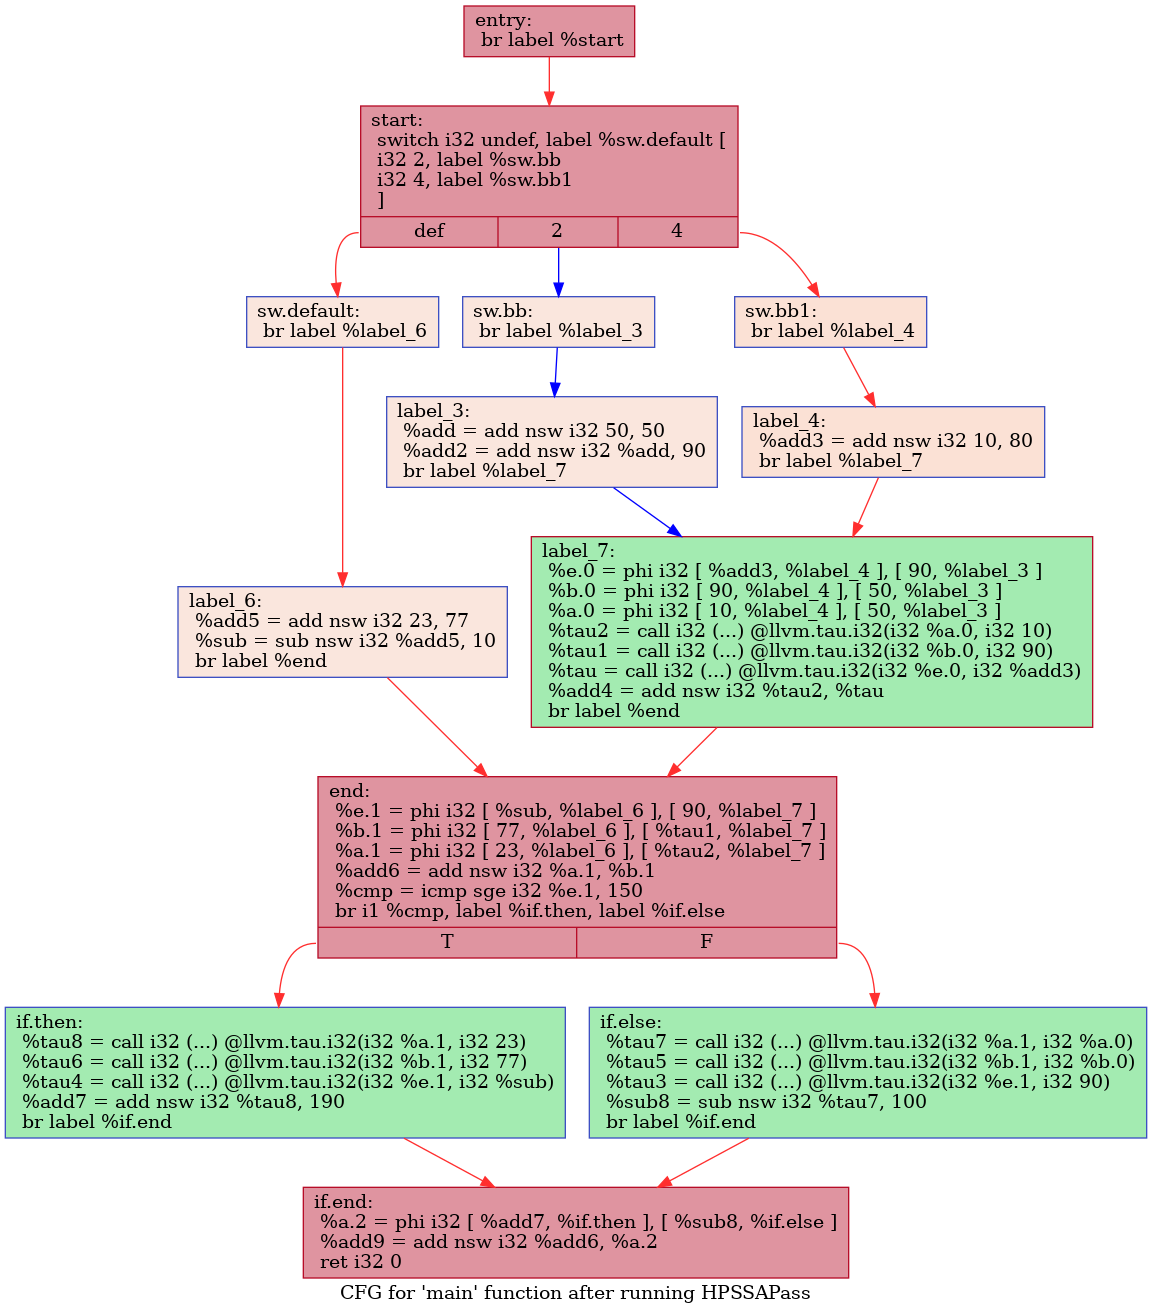
\includegraphics[width=5.8cm,height=7.5cm]{withHPSSA.dot.png}
\end{frame}

\begin{frame}
	\frametitle{\texttt{HPSSAPass} : Auxilliary Functions}
	\begin{itemize}
		\item \mintinline[fontsize=\footnotesize]{css}{HPSSAPass::getProfileInfo(Function \&F)}
		\item \mintinline[fontsize=\footnotesize]{css}{HPSSAPass::getCaloricConnector(Function \&F)}
		\item \mintinline[fontsize=\footnotesize]{css}{HPSSAPass::Search(BasicBlock \&BB, DomTreeNode \&DTN} 
	\end{itemize}
\end{frame}

\begin{frame}
	\frametitle{\texttt{HPSSAPass} : Main \& Destruction Pass}
	\begin{itemize}
		\item \mintinline[fontsize=\footnotesize]{css}{HPSSAPass::run(Function \&F, FunctionAnalysisManager \&AM)} 
		\item \mintinline[fontsize=\footnotesize]{css}{llvm::Function::RPOT()}.
		\item \mintinline[fontsize=\footnotesize]{css}{llvm::successors()}.
		\item \mintinline[fontsize=\footnotesize]{css}{llvm::DominatorTreeAnalysis} and \mintinline[fontsize=\footnotesize]{css}{llvm::dominates()}.
		\item Replace use of \mintinline[]{css}{phi's} with \mintinline[]{css}{tau} variables using \texttt{renaming} stack.
		\item Out of HPSSA Form. 
	\end{itemize}
\end{frame}

\section{LLVM : SSCCP Pass}

\begin{frame}
	\frametitle{\texttt{SSCCP Pass}}

\end{frame}

\begin{frame}
	\frametitle{LLVM Changes}

\end{frame}


\begin{frame}
	\frametitle{SSCCP with an Example}
	
\end{frame}

\end{document}